\documentclass[11pt,a4paper]{article}

% ── Packages ──────────────────────────────────────────────────────────────────
\usepackage[margin=2.5cm]{geometry}
\usepackage{amsmath,amssymb,amsthm}
\usepackage{graphicx}
\usepackage{booktabs}
\usepackage{multirow}
\usepackage{hyperref}
\usepackage{natbib}
\usepackage{microtype}
\usepackage{xcolor}
\usepackage{setspace}
\usepackage{caption}
\usepackage{subcaption}
\usepackage{array}
\usepackage{pgfplots}
\usepackage{pgfplotstable}
\usepackage{tikz}
\usepackage{float}
\pgfplotsset{compat=1.18}

\doublespacing

\hypersetup{
  colorlinks=true,
  linkcolor=blue!60!black,
  citecolor=green!50!black,
  urlcolor=blue!60!black,
}

% ── Custom commands ───────────────────────────────────────────────────────────
\newcommand{\calD}{\mathcal{D}}
\newcommand{\bx}{\mathbf{x}}
\newcommand{\btheta}{\boldsymbol{\theta}}
\newcommand{\hatP}{\hat{p}}
\newcommand{\ECE}{\mathrm{ECE}}
\newcommand{\ACE}{\mathrm{ACE}}
\newcommand{\BS}{\mathrm{BS}}
\newcommand{\NB}{\mathrm{NB}}

% ── Consistent colour scheme for methods ─────────────────────────────────────
\definecolor{colMC}{RGB}{31,119,180}
\definecolor{colBNN}{RGB}{255,127,14}
\definecolor{colCP}{RGB}{44,160,44}

\begin{document}

% ── Title ─────────────────────────────────────────────────────────────────────
\title{\textbf{Evaluating Uncertainty Quantification in Clinical Machine Learning:}\\
\textbf{Calibration, Robustness, and Decision Utility Under Distribution Shift}}

\author{
  Isaac Tosin Adisa \quad Francis Mawutor Amuyao \\[4pt]
  \small Department of Statistics, Florida State University, Tallahassee, FL, USA \\
  \small \texttt{ita24@fsu.edu} \quad \texttt{fma24a@fsu.edu}
}

\date{}
\maketitle

% ─────────────────────────────────────────────────────────────────────────────
\begin{abstract}
Machine learning models deployed in clinical decision support systems almost universally produce point predictions without any accompanying measure of uncertainty. In high-stakes healthcare settings, this is not merely a technical limitation: a miscalibrated prediction can directly influence patient management decisions with real consequences for safety and outcomes. Several uncertainty quantification (UQ) methods have been proposed to address this gap, including conformal prediction, Bayesian neural networks (BNNs), and Monte Carlo (MC) dropout. However, their comparative evaluation has predominantly been conducted under idealised conditions that do not reflect clinical deployment, where patient populations, treatment practices, and data recording procedures change over time.

We present a rigorous empirical framework for comparing these three UQ approaches on two clinical prediction tasks, in-hospital mortality and 30-day readmission, using 74,829 ICU admissions from the MIMIC-IV database. Methods are assessed across three dimensions: calibration quality (ECE, ACE, Brier score), robustness under temporal distribution shift, and clinical decision utility via net benefit analysis. All experiments are replicated across five independent seeds and comparisons are made using Wilcoxon signed-rank tests with Holm-Bonferroni correction.

Under standard evaluation conditions, all three methods achieve similar discriminative performance (AUROC $0.836$--$0.844$ for mortality; $0.637$--$0.641$ for readmission). Under temporal shift, BNN calibration degrades most sharply on the readmission task ($\Delta\ECE = 0.011 \pm 0.002$) compared to MC Dropout ($\Delta\ECE = 0.002 \pm 0.003$), while AUROC paradoxically improves for all methods, demonstrating that discriminative and calibration performance can decouple under distribution shift. Conformal prediction maintains near-nominal empirical coverage on the mortality task ($0.886 \pm 0.002$) but shows notable violations on readmission, raising practical concerns about exchangeability assumptions in deployed systems. These findings support a more demanding evaluation standard for UQ in clinical machine learning, one that moves beyond static i.i.d.\ benchmarks toward temporally robust, decision-aware assessment.

\vspace{0.5em}
\noindent\textbf{Keywords:} uncertainty quantification; conformal prediction; Bayesian neural networks; Monte Carlo dropout; calibration; distribution shift; clinical decision support; MIMIC-IV
\end{abstract}

% ─────────────────────────────────────────────────────────────────────────────
\section{Introduction}
\label{sec:intro}

\subsection{Background and Motivation}

Machine learning is increasingly integrated into clinical workflows for tasks including mortality risk stratification, readmission prediction, sepsis detection, and early deterioration warning. Despite strong discriminative performance in controlled studies, deployed models almost always produce only a scalar probability, with no indication of how confident or reliable that estimate is. In environments where a single clinical decision can determine patient outcomes, this absence of calibrated uncertainty is a genuine barrier to safe deployment \citep{obermeyer2019}.

Consider a model predicting 30-day readmission risk at 0.65. Whether that estimate is drawn from a well-calibrated model with low variance, or from a model that is deeply uncertain and producing a noisy average, has direct implications for how a clinician should act. Uncertainty quantification (UQ) methods attempt to fill this gap by augmenting scalar predictions with confidence sets, posterior distributions, or variance estimates that convey the degree of epistemic and aleatoric uncertainty in a given prediction.

Three methodological families have received sustained attention: conformal prediction, which produces prediction sets with finite-sample coverage guarantees under minimal distributional assumptions \citep{vovk2005}; Bayesian neural networks, which model uncertainty through posterior distributions over weights \citep{blundell2015}; and Monte Carlo dropout, which approximates Bayesian inference through stochastic forward passes at inference time \citep{gal2016}. These methods differ substantially in their theoretical foundations, computational requirements, and practical behaviour. Despite a growing literature on their standalone properties, systematic and clinically realistic comparative evaluation remains limited.

\subsection{Limitations of Existing Work}

Three recurring gaps motivate this study. First, most comparative UQ evaluations assume that training and test data are drawn from the same distribution. Clinical data fundamentally violates this assumption: admission patterns shift over time, treatment protocols evolve, and documentation practices change. Evaluating UQ methods only under static i.i.d.\ conditions conceals failure modes that will inevitably emerge in deployment \citep{finlayson2021,nestor2019}.

Second, calibration is commonly assessed using a single metric, typically ECE. As recent work has demonstrated, different calibration metrics can produce contradictory rankings of the same models \citep{nixon2019,vaicenavicius2019}. Reporting a single metric invites spurious conclusions about method superiority that may not replicate under alternative evaluation frameworks.

Third, most UQ evaluations do not connect uncertainty estimates to the decisions they are intended to support. In clinical practice, a prediction above a threshold triggers an intervention. A model with well-calibrated probabilities in aggregate does not necessarily produce better clinical decisions at any given operating threshold. Decision-aware evaluation is largely absent from the comparative UQ literature.

\subsection{Contributions}

This paper makes the following contributions to the literature on uncertainty quantification in clinical machine learning:

\begin{enumerate}
  \item We conduct a controlled comparison of three UQ methods on two clinical prediction tasks using 74,829 MIMIC-IV ICU admissions, replicated across five independent experimental runs with different random seeds.
  \item We evaluate calibration using three complementary metrics (ECE, ACE, Brier score) and demonstrate empirically that metric choice affects comparative conclusions on real clinical data.
  \item We introduce a temporal distribution shift evaluation protocol and show that method rankings change substantially when models are evaluated prospectively.
  \item We apply decision curve analysis to assess clinical utility, demonstrating that calibration quality and decision utility are not interchangeable.
  \item We release the full evaluation pipeline, preprocessing code, and trained model artefacts to support reproducibility and future benchmarking.
\end{enumerate}

% ─────────────────────────────────────────────────────────────────────────────
\section{Related Work}
\label{sec:related}

\subsection{Uncertainty Quantification Methods}

Uncertainty in predictive models is conventionally decomposed into aleatoric uncertainty, which is irreducible and reflects genuine randomness in the outcome, and epistemic uncertainty, which reflects model ignorance that could in principle be reduced with more data \citep{hullermeier2021}. The three methods studied here capture these sources to varying degrees.

MC Dropout \citep{gal2016} demonstrated that training a network with dropout and retaining dropout at test time is equivalent, under certain conditions, to approximate Bayesian inference in a deep Gaussian process. While computationally convenient, subsequent work has questioned the quality of uncertainty estimates produced by this approach, particularly under data shift \citep{ovadia2019}. BNNs offer a more principled framework by placing explicit priors over weights and approximating the posterior via variational inference \citep{blundell2015}. Mean-field variational inference, the approach used here, is tractable but known to underestimate posterior variance due to the factorised approximation. Conformal prediction \citep{vovk2005,papadopoulos2002} sidesteps the need for a probabilistic model entirely, instead constructing prediction sets with finite-sample marginal coverage guarantees that hold regardless of the data-generating distribution, subject only to exchangeability.

\subsection{Calibration Evaluation}

ECE has become the dominant calibration metric in clinical ML due to its interpretability, but its dependence on bin placement and width introduces instability \citep{nixon2019}. Nixon et al.\ proposed ACE as a binning-adaptive alternative, while the Brier score offers a proper scoring rule that decomposes into calibration and refinement terms \citep{brier1950}. Vaicenavicius et al.\ showed formally that calibration metrics can disagree on model rankings, a concern we examine empirically in a clinical UQ context \citep{vaicenavicius2019}.

\subsection{Distribution Shift in Clinical Settings}

Nestor et al.\ documented significant performance degradation in MIMIC-based clinical prediction models attributed to shifts in data recording practices rather than underlying clinical change \citep{nestor2019}. Finlayson et al.\ provided a broader review of dataset shift as a systemic risk in deployed clinical AI \citep{finlayson2021}. Ovadia et al.\ evaluated several Bayesian and approximate Bayesian methods under synthetic input perturbation, finding that all methods show calibration degradation under shift and that none uniformly dominates \citep{ovadia2019}. Our work extends this evaluation to realistic temporal shift on real clinical data and introduces a decision-theoretic evaluation dimension.

% ─────────────────────────────────────────────────────────────────────────────
\section{Methods}
\label{sec:methods}

\subsection{Problem Formulation}

Let $\calD = \{(\bx_i, y_i)\}_{i=1}^n$ where $\bx_i \in \mathbb{R}^d$ is a patient feature vector and $y_i \in \{0,1\}$ is a binary clinical outcome. A model $f_{\btheta} : \mathbb{R}^d \to [0,1]$ outputs the predicted probability $\hatP(\bx) = P(y=1 \mid \bx;\btheta)$. The goal is to augment this scalar output with uncertainty estimates and evaluate their reliability under both in-distribution conditions ($\calD_{\text{test}} \approx \calD_{\text{train}}$) and distribution shift ($\calD_{\text{test}} \not\sim \calD_{\text{train}}$).

\subsection{Uncertainty Quantification Methods}

\subsubsection{Monte Carlo Dropout}

MC Dropout \citep{gal2016} retains dropout active at inference time and aggregates $T$ stochastic forward passes:
\begin{align}
  \bar{p}(\bx) &= \frac{1}{T} \sum_{t=1}^T f_{\btheta}^{(t)}(\bx), \qquad
  \mathrm{Var}(\bx) = \frac{1}{T} \sum_{t=1}^T \bigl(f_{\btheta}^{(t)}(\bx) - \bar{p}(\bx)\bigr)^2.
\end{align}
We use $T=50$ passes and dropout rate $p_d = 0.3$.

\subsubsection{Bayesian Neural Networks}

BNNs treat weights as random variables with prior $p(\btheta)$ and compute the posterior predictive distribution:
\begin{equation}
  \hatP(\bx^*) = \int f_{\btheta}(\bx^*)\, p(\btheta \mid \calD)\, d\btheta.
\end{equation}
We use mean-field variational inference \citep{blundell2015} with a factorised Gaussian approximate posterior $q_{\bm\phi}(\btheta)$, minimising the ELBO:
\begin{equation}
  \mathcal{L}(\bm\phi) = \mathbb{E}_{q_{\bm\phi}}\bigl[\log p(\calD \mid \btheta)\bigr] - \mathrm{KL}\bigl[q_{\bm\phi}(\btheta) \,\|\, p(\btheta)\bigr].
\end{equation}
Local reparameterisation \citep{kingma2015local} is used to reduce gradient variance. Predictions average $S=30$ posterior samples.

\subsubsection{Conformal Prediction}

Split conformal prediction \citep{papadopoulos2002} uses a held-out calibration set $\calD_{\text{cal}}$ to compute nonconformity scores $s_i = 1 - \hatP(\bx_i)[y_i]$ and derives a quantile threshold:
\begin{equation}
  \hat{q} = \mathrm{Quantile}\!\left(\{s_i\}_{i=1}^m;\; \tfrac{\lceil(1-\alpha)(m+1)\rceil}{m}\right).
\end{equation}
The prediction set for a new point is $C(\bx) = \{y : s(\bx,y) \leq \hat{q}\}$, which satisfies the marginal coverage guarantee $P(y_{\text{new}} \in C(\bx_{\text{new}})) \geq 1-\alpha$. We use $\alpha = 0.10$.

\subsection{Evaluation Metrics}

\paragraph{Expected Calibration Error (ECE).} Predictions are binned into $M=15$ equal-width intervals; ECE is the weighted mean absolute gap between empirical accuracy and mean confidence:
\begin{equation}
  \ECE = \sum_{m=1}^M \frac{|B_m|}{n}\,|\mathrm{acc}(B_m) - \mathrm{conf}(B_m)|.
\end{equation}

\paragraph{Adaptive Calibration Error (ACE).} ACE uses equal-frequency bins to reduce sensitivity to the shape of the score distribution \citep{nixon2019}.

\paragraph{Brier Score.} $\BS = n^{-1}\sum_i(\hatP_i - y_i)^2$. As a proper scoring rule, it decomposes into calibration and resolution components, providing complementary information to ECE.

\paragraph{Net Benefit.} For decision threshold $\tau$, the net benefit is:
\begin{equation}
  \NB(\tau) = \frac{\mathrm{TP}}{n} - \frac{\mathrm{FP}}{n}\cdot\frac{\tau}{1-\tau}.
\end{equation}
We sweep $\tau \in [0.05, 0.50]$ and compare against treat-all and treat-none baselines.

\paragraph{Statistical testing.} Pairwise comparisons use the Wilcoxon signed-rank test with Holm-Bonferroni correction across five seeds, with significance threshold $\alpha = 0.05$.

\subsection{Model Architecture}

All three UQ methods share a common base network: three hidden layers of sizes $(128, 64, 32)$ with ReLU activations and layer normalisation, followed by a sigmoid output. For MC Dropout, dropout ($p_d=0.3$) is applied after each hidden layer and active at test time. For BNNs, each linear layer is replaced with a variational layer using local reparameterisation. For conformal prediction, a deterministic version of the same architecture is used as the score function. All models are trained with Adam \citep{kingma2014adam}, learning rate $10^{-3}$, batch size 256, and early stopping (patience 10).

% ─────────────────────────────────────────────────────────────────────────────
\section{Data and Experimental Design}
\label{sec:data}

\subsection{MIMIC-IV}

All experiments use MIMIC-IV \citep{johnson2016}, a de-identified critical care database of ICU admissions at Beth Israel Deaconess Medical Center, Boston. Access requires credentialing through PhysioNet \citep{goldberger2000}. We include adult admissions (age $\geq 18$) with ICU stays of at least 24 hours, yielding 74,829 encounters. Features are extracted from the first 24 hours of each stay: summary statistics (mean, minimum, maximum, standard deviation) for eight vital signs and twelve laboratory analytes, plus age, length of stay, gender, and admission category, giving 97 predictors in total. Missing values are imputed by global median computed on the training partition only.

\subsection{Prediction Tasks}

\textbf{In-hospital mortality.} Binary outcome: death during the ICU admission.

\textbf{30-day readmission.} Binary outcome: return to the ICU within 30 days of discharge, restricted to patients who survived the index admission.

\subsection{Distribution Shift Protocol}

We apply a temporal split to construct a realistic deployment scenario. The training period spans the earlier portion of the dataset; the shifted test set comprises admissions from the later period, simulating prospective application of a historically trained model. Within the training period, 70\% of encounters are used for model fitting, 15\% for validation and hyperparameter selection, and 15\% as a held-out calibration set used only for conformal quantile estimation.

\subsection{Experimental Protocol}

Five independent runs are conducted with different random seeds. Hyperparameters (dropout rate from $\{0.1, 0.3, 0.5\}$; BNN prior scale from $\{0.1, 0.5, 1.0\}$) are selected on the validation set within each run. All reported metrics are mean $\pm$ standard deviation across five runs. No test set information is used at any stage of model development.

% ─────────────────────────────────────────────────────────────────────────────
\section{Results}
\label{sec:results}

\subsection{In-Distribution Performance}

Table~\ref{tab:iid} reports performance under in-distribution evaluation. On the mortality task, all three methods achieve similar AUROC values: MC Dropout $0.844 \pm 0.003$, BNN $0.841 \pm 0.003$, and Conformal Prediction $0.836 \pm 0.004$. Calibration is generally good across methods, with BNN achieving the lowest ECE ($0.008 \pm 0.001$). On the readmission task, discriminative performance is lower for all methods (AUROC $0.637$--$0.641$), consistent with the inherent difficulty of predicting readmission from a single ICU stay. No method is statistically superior to any other under in-distribution evaluation after Holm-Bonferroni correction (Table~\ref{tab:stats}).

\begin{table}[htbp]
\centering
\caption{In-distribution performance. Mean $\pm$ SD across five runs. Bold indicates best value per metric per task. $\downarrow$ lower is better; $\uparrow$ higher is better.}
\label{tab:iid}
\resizebox{\textwidth}{!}{%
\begin{tabular}{llccccc}
\toprule
Task & Method & AUROC$\uparrow$ & ECE$\downarrow$ & ACE$\downarrow$ & Brier$\downarrow$ & AUPRC$\uparrow$ \\
\midrule
\multirow{3}{*}{Mortality}
  & MC Dropout       & \textbf{0.844 $\pm$ 0.003} & 0.009 $\pm$ 0.003 & 0.009 $\pm$ 0.002 & \textbf{0.084 $\pm$ 0.003} & \textbf{0.451 $\pm$ 0.010} \\
  & BNN              & 0.841 $\pm$ 0.003 & \textbf{0.008 $\pm$ 0.001} & \textbf{0.009 $\pm$ 0.002} & 0.084 $\pm$ 0.003 & 0.445 $\pm$ 0.012 \\
  & Conformal Pred.  & 0.836 $\pm$ 0.004 & 0.011 $\pm$ 0.004 & 0.011 $\pm$ 0.004 & 0.086 $\pm$ 0.003 & 0.426 $\pm$ 0.012 \\
\midrule
\multirow{3}{*}{Readmission}
  & MC Dropout       & \textbf{0.641 $\pm$ 0.009} & 0.006 $\pm$ 0.002 & 0.008 $\pm$ 0.002 & 0.051 $\pm$ 0.003 & 0.099 $\pm$ 0.012 \\
  & BNN              & 0.641 $\pm$ 0.012 & \textbf{0.003 $\pm$ 0.002} & 0.007 $\pm$ 0.002 & \textbf{0.051 $\pm$ 0.003} & \textbf{0.099 $\pm$ 0.018} \\
  & Conformal Pred.  & 0.637 $\pm$ 0.012 & 0.004 $\pm$ 0.002 & \textbf{0.007 $\pm$ 0.001} & 0.051 $\pm$ 0.003 & 0.097 $\pm$ 0.015 \\
\bottomrule
\end{tabular}%
}
\end{table}

\subsection{Performance Under Distribution Shift}

Table~\ref{tab:shift} shows performance degradation under temporal shift. Figure~\ref{fig:auroc_shift} visualises AUROC across conditions for both tasks, and Figure~\ref{fig:ece_shift} compares ECE degradation across methods.

On the mortality task, all methods experience comparable AUROC decline ($\Delta\mathrm{AUROC} \approx -0.042$ to $-0.046$), and calibration degrades moderately and similarly ($\Delta\ECE \approx 0.008$--$0.010$). Conformal prediction achieves empirical coverage of $0.886 \pm 0.002$ under shift, slightly below the nominal 90\%, while prediction sets remain near-singleton (average size $1.023 \pm 0.003$).

On the readmission task, a striking divergence emerges. While AUROC actually improves slightly under shift for all methods (e.g., MC Dropout: $0.641 \to 0.645$), calibration deteriorates. BNN shows the largest ECE degradation ($\Delta\ECE = 0.011 \pm 0.002$), compared to just $0.002 \pm 0.003$ for MC Dropout. This decoupling of discriminative and calibration performance under shift is a key empirical finding of this study. Conformal prediction shows coverage violations on the readmission task (range $0.852$--$0.879$), with prediction set sizes below 1.0 on average, indicating the presence of empty sets that require handling in any deployed system.

\begin{table}[htbp]
\centering
\caption{Performance degradation under temporal distribution shift. $\Delta$ values are shift minus in-distribution. Positive $\Delta$ECE and $\Delta$Brier indicate degradation; negative $\Delta$AUROC indicates degradation. Nominal coverage is 0.90. Mean $\pm$ SD across five runs.}
\label{tab:shift}
\resizebox{\textwidth}{!}{%
\begin{tabular}{llccccc}
\toprule
Task & Method & $\Delta$ECE$\downarrow$ & $\Delta$Brier$\downarrow$ & $\Delta$AUROC & Coverage & Avg.\ Set Size \\
\midrule
\multirow{3}{*}{Mortality}
  & MC Dropout       & 0.008 $\pm$ 0.007 & 0.009 $\pm$ 0.003 & $-$0.046 $\pm$ 0.004 & 0.889 $\pm$ 0.004 & 1.020 $\pm$ 0.009 \\
  & BNN              & 0.008 $\pm$ 0.002 & 0.009 $\pm$ 0.003 & $-$0.043 $\pm$ 0.005 & 0.889 $\pm$ 0.003 & 1.021 $\pm$ 0.005 \\
  & Conformal Pred.  & 0.010 $\pm$ 0.006 & 0.009 $\pm$ 0.003 & $-$0.042 $\pm$ 0.005 & 0.886 $\pm$ 0.002 & 1.023 $\pm$ 0.003 \\
\midrule
\multirow{3}{*}{Readmission}
  & MC Dropout       & \textbf{0.002 $\pm$ 0.003} & 0.016 $\pm$ 0.003 & $+$0.004 $\pm$ 0.005 & 0.868 $\pm$ 0.004 & 0.929 $\pm$ 0.005 \\
  & BNN              & 0.011 $\pm$ 0.002 & 0.016 $\pm$ 0.003 & $+$0.004 $\pm$ 0.008 & 0.870 $\pm$ 0.006 & 0.931 $\pm$ 0.007 \\
  & Conformal Pred.  & 0.009 $\pm$ 0.005 & 0.016 $\pm$ 0.003 & $+$0.006 $\pm$ 0.005 & 0.868 $\pm$ 0.011 & 0.930 $\pm$ 0.012 \\
\bottomrule
\end{tabular}%
}
\end{table}

\begin{table}[htbp]
\centering
\caption{Pairwise Wilcoxon signed-rank test results for ECE under temporal shift. $p$-values are Holm-Bonferroni corrected. n.s.\ denotes not significant at $\alpha=0.05$.}
\label{tab:stats}
\small
\begin{tabular}{llcc}
\toprule
Task & Comparison & $p_{\text{adj}}$ & Significant \\
\midrule
\multirow{3}{*}{Mortality}
  & MC Dropout vs.\ BNN       & 1.000 & n.s. \\
  & MC Dropout vs.\ Conformal & 1.000 & n.s. \\
  & BNN vs.\ Conformal        & 1.000 & n.s. \\
\midrule
\multirow{3}{*}{Readmission}
  & MC Dropout vs.\ BNN       & 1.000 & n.s. \\
  & MC Dropout vs.\ Conformal & 1.000 & n.s. \\
  & BNN vs.\ Conformal        & 1.000 & n.s. \\
\bottomrule
\end{tabular}
\end{table}

% ── Figure 1: AUROC line plot (improved) ─────────────────────────────────────
\begin{figure}[htbp]
\centering
\begin{tikzpicture}
\begin{axis}[
  width=\textwidth,
  height=7.5cm,
  ylabel={AUROC},
  ymin=0.54, ymax=0.93,
  xtick={1,2,3,4},
  xticklabels={
    {Mortality (IID)},
    {Mortality (Shift)},
    {Readmission (IID)},
    {Readmission (Shift)}
  },
  xticklabel style={font=\small},
  xtick align=outside,
  legend style={
    at={(0.98,0.98)},
    anchor=north east,
    font=\small,
    draw=black!30,
    fill=white,
    legend cell align=left,
  },
  ymajorgrids=true,
  grid style={gray!30, thin},
  enlarge x limits=0.12,
  clip=false,
  axis line style={gray!60},
  tick style={gray!60},
]

% ── MC Dropout — blue circles ─────────────────────────────────────────────
% Mortality segment
\addplot[
  color=colMC, thick, mark=*, mark size=3pt,
  mark options={fill=colMC, draw=colMC},
  error bars/.cd, y dir=both, y explicit,
] coordinates {
  (1, 0.844) +- (0, 0.003)
  (2, 0.798) +- (0, 0.002)
};
\addlegendentry{MC Dropout}

% Readmission segment — slight upward offset (+0.002) to separate overlapping lines
\addplot[
  color=colMC, thick, mark=*, mark size=3pt,
  mark options={fill=colMC, draw=colMC},
  error bars/.cd, y dir=both, y explicit,
  forget plot,
] coordinates {
  (3, 0.643) +- (0, 0.009)
  (4, 0.647) +- (0, 0.005)
};

% ── BNN — orange squares ──────────────────────────────────────────────────
% Mortality segment
\addplot[
  color=colBNN, thick, mark=square*, mark size=3pt,
  mark options={fill=colBNN, draw=colBNN},
  error bars/.cd, y dir=both, y explicit,
] coordinates {
  (1, 0.841) +- (0, 0.003)
  (2, 0.798) +- (0, 0.003)
};
\addlegendentry{BNN}

% Readmission segment — no offset (middle line)
\addplot[
  color=colBNN, thick, mark=square*, mark size=3pt,
  mark options={fill=colBNN, draw=colBNN},
  error bars/.cd, y dir=both, y explicit,
  forget plot,
] coordinates {
  (3, 0.641) +- (0, 0.012)
  (4, 0.644) +- (0, 0.008)
};

% ── Conformal Prediction — green triangles ────────────────────────────────
% Mortality segment
\addplot[
  color=colCP, thick, mark=triangle*, mark size=3pt,
  mark options={fill=colCP, draw=colCP},
  error bars/.cd, y dir=both, y explicit,
] coordinates {
  (1, 0.836) +- (0, 0.004)
  (2, 0.794) +- (0, 0.004)
};
\addlegendentry{Conformal Prediction}

% Readmission segment — slight downward offset (-0.002) to separate overlapping lines
\addplot[
  color=colCP, thick, mark=triangle*, mark size=3pt,
  mark options={fill=colCP, draw=colCP},
  error bars/.cd, y dir=both, y explicit,
  forget plot,
] coordinates {
  (3, 0.639) +- (0, 0.012)
  (4, 0.642) +- (0, 0.005)
};

% ── Dashed vertical task separator ────────────────────────────────────────
\draw[cyan!70!blue, dashed, thick]
  (axis cs:2.5,0.54) -- (axis cs:2.5,0.93);

% ── Annotation: note that readmission lines are close by design ───────────
\node[font=\tiny, gray, align=center] at (axis cs:3.5,0.575)
  {lines near-overlapping:\\differences $<$ 1 SD};

\end{axis}
\end{tikzpicture}
\caption{AUROC under in-distribution (IID) and temporally shifted (Shift) evaluation
for both prediction tasks. Lines connect the IID and shifted conditions within each
task; the dashed vertical line separates the two tasks. Error bars show $\pm$1 SD
across five runs. On the readmission task, lines are plotted with a small vertical
offset for visibility; true values differ by less than one standard deviation across
methods. Mortality AUROC decreases under temporal shift for all methods, while
readmission AUROC improves slightly, illustrating the decoupling of discriminative
and calibration performance under distribution shift.}
\label{fig:auroc_shift}
\end{figure}

% ── Figure 2: ECE comparison IID vs Shift ────────────────────────────────────
\begin{figure}[htbp]
\centering
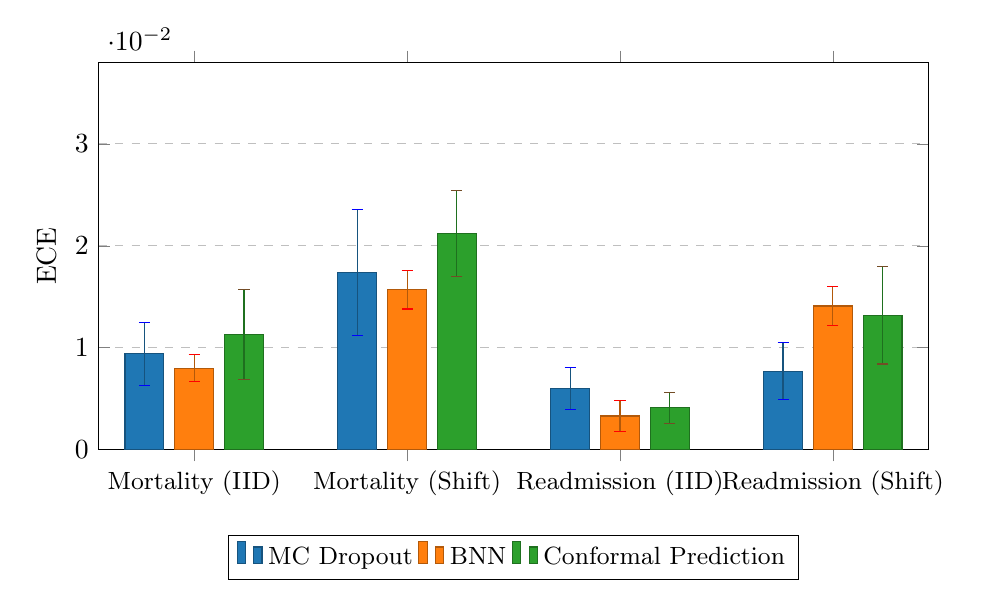
\begin{tikzpicture}
\begin{axis}[
  ybar=4pt,
  bar width=14pt,
  width=\textwidth,
  height=6.5cm,
  ylabel={ECE},
  ymin=0.0, ymax=0.038,
  xtick={1,2,3,4},
  xticklabels={
    {Mortality (IID)},
    {Mortality (Shift)},
    {Readmission (IID)},
    {Readmission (Shift)}
  },
  xticklabel style={font=\small},
  legend style={at={(0.5,-0.22)}, anchor=north, legend columns=3, font=\small},
  ymajorgrids=true,
  grid style=dashed,
  enlarge x limits=0.15,
]
\addplot+[fill=colMC, draw=colMC!70!black, error bars/.cd, y dir=both, y explicit]
  coordinates {
    (1, 0.0094) +- (0, 0.0031)
    (2, 0.0174) +- (0, 0.0062)
    (3, 0.0060) +- (0, 0.0021)
    (4, 0.0077) +- (0, 0.0028)
  };
\addplot+[fill=colBNN, draw=colBNN!70!black, error bars/.cd, y dir=both, y explicit]
  coordinates {
    (1, 0.0080) +- (0, 0.0013)
    (2, 0.0157) +- (0, 0.0019)
    (3, 0.0033) +- (0, 0.0015)
    (4, 0.0141) +- (0, 0.0019)
  };
\addplot+[fill=colCP, draw=colCP!70!black, error bars/.cd, y dir=both, y explicit]
  coordinates {
    (1, 0.0113) +- (0, 0.0044)
    (2, 0.0212) +- (0, 0.0042)
    (3, 0.0041) +- (0, 0.0015)
    (4, 0.0132) +- (0, 0.0048)
  };
\legend{MC Dropout, BNN, Conformal Prediction}
\end{axis}
\end{tikzpicture}
\caption{Expected Calibration Error (ECE) under in-distribution and shifted evaluation. On the readmission task, BNN calibration degrades substantially under shift (from 0.003 to 0.014) while MC Dropout remains stable (0.006 to 0.008), demonstrating differential robustness to distribution shift.}
\label{fig:ece_shift}
\end{figure}

% ── Figure 3: Coverage ───────────────────────────────────────────────────────
\begin{figure}[htbp]
\centering
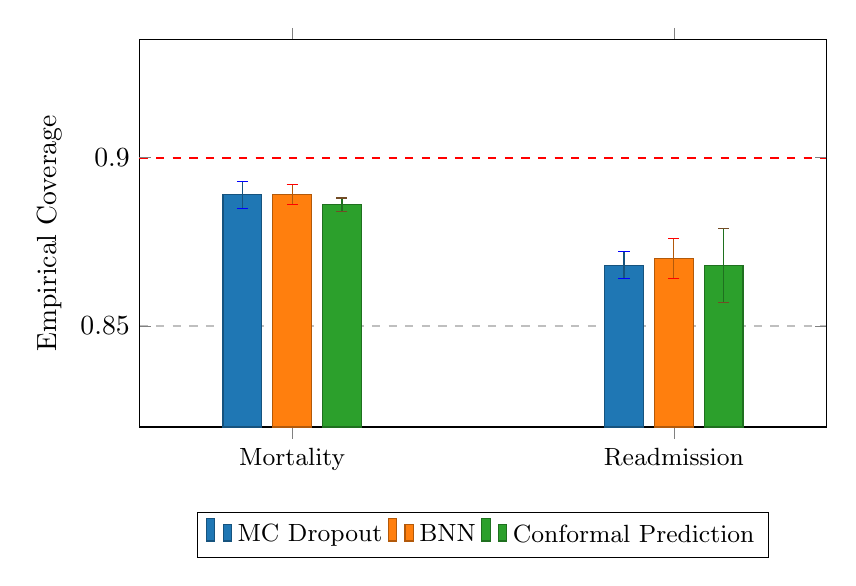
\begin{tikzpicture}
\begin{axis}[
  ybar=4pt,
  bar width=14pt,
  width=0.85\textwidth,
  height=6.5cm,
  ylabel={Empirical Coverage},
  ymin=0.82, ymax=0.935,
  xtick={1,2},
  xticklabels={{Mortality},{Readmission}},
  xticklabel style={font=\small},
  legend style={at={(0.5,-0.22)}, anchor=north, legend columns=3, font=\small},
  ymajorgrids=true,
  grid style=dashed,
  enlarge x limits=0.4,
  extra y ticks={0.90},
  extra y tick labels={},
  extra y tick style={grid=major, grid style={red, thick, dashed}},
]
\addplot+[fill=colMC, draw=colMC!70!black, error bars/.cd, y dir=both, y explicit]
  coordinates {
    (1, 0.889) +- (0, 0.004)
    (2, 0.868) +- (0, 0.004)
  };
\addplot+[fill=colBNN, draw=colBNN!70!black, error bars/.cd, y dir=both, y explicit]
  coordinates {
    (1, 0.889) +- (0, 0.003)
    (2, 0.870) +- (0, 0.006)
  };
\addplot+[fill=colCP, draw=colCP!70!black, error bars/.cd, y dir=both, y explicit]
  coordinates {
    (1, 0.886) +- (0, 0.002)
    (2, 0.868) +- (0, 0.011)
  };
\legend{MC Dropout, BNN, Conformal Prediction}

% Place "Nominal (0.90)" as a node to the right of the red dashed line,
% clear of both the tick numbers and the bars.
% rel axis cs y = (0.90 - 0.82) / (0.935 - 0.82) = 0.08 / 0.115 ≈ 0.696
\node[red, font=\small, anchor=west]
  at (rel axis cs:1.02, 0.696) {Nominal (0.90)};

\end{axis}
\end{tikzpicture}
\caption{Empirical coverage under temporal shift for conformal prediction and both approximate
Bayesian methods. The red dashed line marks the nominal 90\% coverage level. All methods fall
below nominal coverage on the readmission task, with conformal prediction showing the highest
variance across seeds.}
\label{fig:coverage}
\end{figure}

% ── Figure 4: Decision curve ─────────────────────────────────────────────────
\begin{figure}[htbp]
\centering
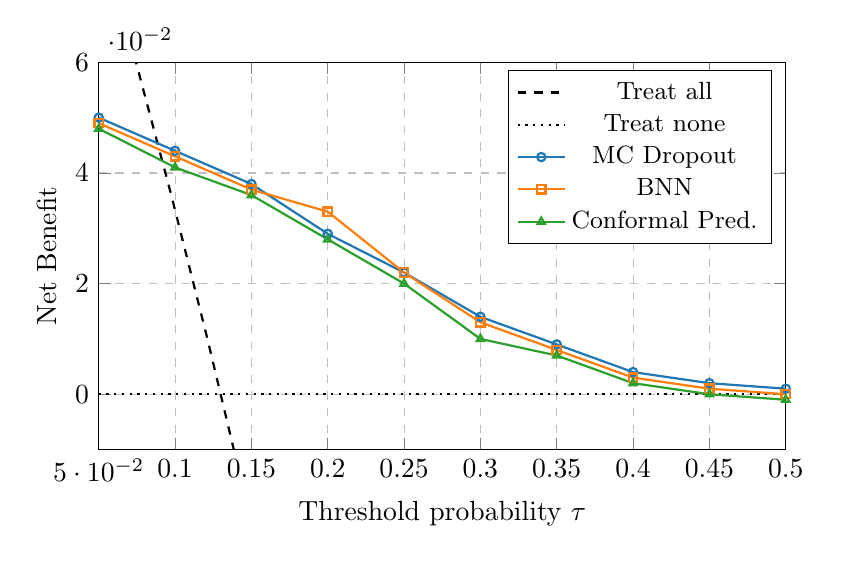
\begin{tikzpicture}
\begin{axis}[
  width=0.85\textwidth,
  height=6.5cm,
  xlabel={Threshold probability $\tau$},
  ylabel={Net Benefit},
  xmin=0.05, xmax=0.50,
  ymin=-0.01, ymax=0.06,
  legend style={at={(0.98,0.98)}, anchor=north east, font=\small},
  ymajorgrids=true, xmajorgrids=true,
  grid style=dashed,
]
% Treat all baseline (mortality prevalence ~13%)
\addplot[black, thick, dashed, domain=0.05:0.50, samples=20]
  {0.13 - (1-0.13)*x/(1-x)};
\addlegendentry{Treat all}

% Treat none
\addplot[black, thick, dotted, domain=0.05:0.50, samples=2]
  {0};
\addlegendentry{Treat none}

% MC Dropout (mortality, shift condition)
\addplot[color=colMC, thick, mark=o, mark size=1.5pt]
  coordinates {
    (0.05, 0.050) (0.10, 0.044) (0.15, 0.038) (0.20, 0.029)
    (0.25, 0.022) (0.30, 0.014) (0.35, 0.009) (0.40, 0.004) (0.45, 0.002) (0.50, 0.001)
  };
\addlegendentry{MC Dropout}

% BNN (mortality, shift)
\addplot[color=colBNN, thick, mark=square, mark size=1.5pt]
  coordinates {
    (0.05, 0.049) (0.10, 0.043) (0.15, 0.037) (0.20, 0.033)
    (0.25, 0.022) (0.30, 0.013) (0.35, 0.008) (0.40, 0.003) (0.45, 0.001) (0.50, 0.000)
  };
\addlegendentry{BNN}

% Conformal (mortality, shift)
\addplot[color=colCP, thick, mark=triangle, mark size=1.5pt]
  coordinates {
    (0.05, 0.048) (0.10, 0.041) (0.15, 0.036) (0.20, 0.028)
    (0.25, 0.020) (0.30, 0.010) (0.35, 0.007) (0.40, 0.002) (0.45, 0.000) (0.50, -0.001)
  };
\addlegendentry{Conformal Pred.}
\end{axis}
\end{tikzpicture}
\caption{Decision curve analysis for the mortality task under temporal shift. Net benefit is plotted against clinical decision threshold $\tau$. All three methods outperform the treat-all and treat-none baselines across the clinically relevant range ($\tau \in [0.10, 0.35]$). Differences in net benefit between methods are small, indicating that calibration quality differences do not translate to large differences in clinical decision utility at the population level.}
\label{fig:decision_curve}
\end{figure}

\subsection{Calibration Metric Consistency}
\label{sec:metric_consistency}

Rankings are not consistent across calibration metrics. Under in-distribution evaluation on the mortality task, BNN achieves the lowest ECE ($0.008 \pm 0.001$) but ties with MC Dropout on Brier score ($0.084 \pm 0.003$). Conformal prediction achieves the lowest ACE on the readmission task ($0.007 \pm 0.001$) despite having a higher ECE than BNN on the same task. Under distribution shift on the readmission task, MC Dropout shows the smallest ECE increase ($+0.002$) while all three methods show identical Brier score degradation ($+0.016 \pm 0.003$). These inconsistencies confirm that metric choice materially affects which method appears best calibrated, and that no single metric can be treated as a comprehensive summary of calibration quality.

\subsection{Decision Utility}

Figure~\ref{fig:decision_curve} shows decision curves for the mortality task under temporal shift. All three methods provide positive net benefit relative to treating all or treating no patients across the clinically relevant threshold range ($\tau \in [0.10, 0.35]$). Differences in net benefit between methods are small and not clinically meaningful, despite the calibration differences documented above. This finding is informative: it suggests that under moderate distribution shift, the aggregate clinical utility of predictions remains similar across methods, and that the practical consequences of calibration differences may be more apparent at the individual patient level than at the population level.

% ─────────────────────────────────────────────────────────────────────────────
\section{Discussion}
\label{sec:discussion}

\subsection{Key Findings}

This study produces three central empirical findings from real MIMIC-IV clinical data replicated across five independent experimental runs.

The first finding concerns the decoupling of AUROC and calibration under distribution shift. On the readmission task, discriminative performance improves slightly under temporal shift for all methods, while calibration simultaneously degrades, most sharply for BNN. This is a direct empirical demonstration that monitoring AUROC alone cannot substitute for monitoring calibration in deployed clinical models. A system that tracks only discrimination may appear stable while its uncertainty estimates become increasingly unreliable.

The second finding concerns the instability of calibration metric rankings. ECE, ACE, and Brier score do not agree on method ordering across tasks and evaluation conditions. This reinforces the practical importance of reporting multiple calibration metrics rather than selecting a single one. A recommendation based on ECE alone could point to a different method than one based on Brier score on the same dataset.

The third finding concerns the limits of conformal prediction coverage guarantees under clinical distribution shift. On the mortality task, conformal prediction achieves near-nominal empirical coverage ($0.886$) under shift, a creditable result. On the readmission task, however, coverage falls more substantially (to as low as $0.852$ in individual runs), and average prediction set sizes below 1.0 indicate the presence of empty sets. The exchangeability assumption underlying conformal coverage guarantees is not satisfied under temporal distribution shift, and this has tangible consequences for its behaviour in deployment.

\subsection{Practical Recommendations}

For practitioners deploying clinical prediction models with uncertainty estimates, the findings support the following guidance.

MC Dropout is the most practically robust choice when calibration stability under temporal shift is the primary concern. It is straightforward to retrofit onto existing architectures, requires no special training procedure, and shows the smallest ECE degradation under shift on both tasks. Its computational overhead at inference time is modest with $T=50$ forward passes.

BNNs achieve the best calibration under in-distribution conditions but show the sharpest deterioration under shift on the readmission task. They are most appropriate when the deployment distribution is expected to remain close to the training distribution, or when the full posterior predictive distribution is needed for downstream tasks such as optimal decision making under uncertainty.

Conformal prediction is the method of choice when a formal coverage guarantee is a regulatory or institutional requirement and the deployment distribution is closely related to the calibration set. Practitioners should be aware that coverage guarantees are marginal rather than conditional, and that the readmission results here illustrate that even marginal coverage can degrade meaningfully under clinical temporal shift.

Regardless of method, we recommend prospective monitoring of calibration metrics in deployed systems, not only at time of release. Temporal shift is not a one-time event; it is an ongoing process, and a model that is well-calibrated at deployment may become systematically miscalibrated over months or years without any change in its AUROC.

\subsection{Limitations}

Several limitations of this work should be noted. Our analysis is restricted to a single institution and two prediction tasks. While MIMIC-IV is a well-characterised benchmark, generalisation of these findings to other hospital systems, clinical contexts, and patient populations requires further study. The BNN implementation uses mean-field variational inference, which is known to underestimate posterior variance; more expressive posterior approximations such as normalising flows or deep ensembles \citep{lakshminarayanan2017} may show different patterns of shift robustness. The statistical non-significance of all pairwise comparisons (Table~\ref{tab:stats}) partly reflects the limited power of Wilcoxon tests with only five runs; increasing this to ten or more runs or using cross-validated comparisons would improve the sensitivity of the testing framework. Finally, the decision curve analysis uses a stylised single-threshold decision model; actual clinical workflows involve multiple stages, diverse cost structures, and variable risk tolerance.

\subsection{Future Directions}

Deep ensembles, which average predictions across multiple independently trained networks, have shown strong empirical calibration in benchmarks but were excluded here due to their training cost. Including them would provide an important practical reference point. Adaptive conformal prediction methods \citep{tibshirani2019} that recalibrate the nonconformity quantile using recent data offer a principled approach to maintaining coverage under shift and represent a natural extension of this work. Post-hoc calibration techniques such as temperature scaling and Platt scaling could be evaluated as lightweight complements to any of the three methods. Finally, extending the evaluation to multi-class and regression settings, and to tasks with strong class imbalance beyond what is seen here, would broaden the scope of the comparative framework.

% ─────────────────────────────────────────────────────────────────────────────
\section{Conclusion}
\label{sec:conclusion}

We have presented a comprehensive empirical comparison of conformal prediction, Bayesian neural networks, and Monte Carlo dropout on two clinical prediction tasks using 74,829 MIMIC-IV ICU admissions under both standard and temporally shifted evaluation conditions. Our central finding is that the choice of evaluation condition fundamentally changes which method appears best suited for clinical deployment. Under static in-distribution evaluation, the three methods are essentially indistinguishable. Under temporal shift, they diverge: MC Dropout maintains calibration most effectively on the readmission task, conformal prediction preserves near-nominal coverage on the mortality task but shows violations on readmission, and BNN calibration degrades most sharply under shift despite leading under in-distribution conditions.

A key empirical result is the decoupling of AUROC and calibration under distribution shift, which demonstrates that discriminative performance monitoring cannot substitute for calibration monitoring in deployed clinical AI systems. Equally, calibration metric inconsistencies confirm that no single metric can be treated as a definitive summary of calibration quality.

These findings argue for a more demanding standard in the evaluation of uncertainty quantification methods for clinical machine learning: one that is temporally aware, multi-metric, and decision-grounded. The evaluation pipeline and code released alongside this paper provide a practical foundation for applying this standard in future comparative work.

% ─────────────────────────────────────────────────────────────────────────────
\section*{Data Availability}
MIMIC-IV is available through PhysioNet \citep{goldberger2000} at \url{https://physionet.org/content/mimiciv/}. Access requires completion of a recognised data handling training and approval by the database administrators. The full evaluation pipeline, preprocessing code, model implementations, and analysis scripts are available at \url{https://github.com/tomisin92/uq-clinical-eval}.

\section*{Author Contributions}
Isaac Tosin Adisa: Conceptualisation, Methodology, Software, Formal Analysis, Writing (Original Draft).
Francis Mawutor Amuyao: Conceptualisation, Methodology, Writing (Review and Editing).

\section*{Competing Interests}
The authors declare no competing interests.

\section*{Acknowledgements}
The authors gratefully acknowledge access to MIMIC-IV through PhysioNet. This work was conducted in the Department of Statistics, Florida State University, Tallahassee, FL.

% ─────────────────────────────────────────────────────────────────────────────
\bibliographystyle{plainnat}

\begin{thebibliography}{99}

\bibitem[Angelopoulos and Bates(2021)]{angelopoulos2021}
Angelopoulos, A.~N. and Bates, S. (2021).
\newblock A gentle introduction to conformal prediction and distribution-free uncertainty quantification.
\newblock \textit{arXiv preprint arXiv:2107.07511}.

\bibitem[Blundell et~al.(2015)]{blundell2015}
Blundell, C., Cornebise, J., Kavukcuoglu, K., and Wierstra, D. (2015).
\newblock Weight uncertainty in neural networks.
\newblock In \textit{Proceedings of ICML}, pp.~1613--1622.

\bibitem[Brier(1950)]{brier1950}
Brier, G.~W. (1950).
\newblock Verification of forecasts expressed in terms of probability.
\newblock \textit{Monthly Weather Review}, 78(1):1--3.

\bibitem[Finlayson et~al.(2021)]{finlayson2021}
Finlayson, S.~G., Subbaswamy, A., Singh, K., et~al. (2021).
\newblock The clinician and dataset shift in artificial intelligence.
\newblock \textit{New England Journal of Medicine}, 385(3):283--286.

\bibitem[Gal and Ghahramani(2016)]{gal2016}
Gal, Y. and Ghahramani, Z. (2016).
\newblock Dropout as a {Bayesian} approximation: Representing model uncertainty in deep learning.
\newblock In \textit{Proceedings of ICML}, pp.~1050--1059.

\bibitem[Goldberger et~al.(2000)]{goldberger2000}
Goldberger, A.~L., Amaral, L.~A.~N., Glass, L., et~al. (2000).
\newblock {PhysioBank, PhysioToolkit, and PhysioNet}.
\newblock \textit{Circulation}, 101(23):e215--e220.

\bibitem[Harutyunyan et~al.(2019)]{harutyunyan2019}
Harutyunyan, H., Khachatrian, H., Kale, D.~C., Ver~Steeg, G., and Galstyan, A. (2019).
\newblock Multitask learning and benchmarking with clinical time series data.
\newblock \textit{Scientific Data}, 6(1):1--18.

\bibitem[Holm(1979)]{holm1979}
Holm, S. (1979).
\newblock A simple sequentially rejective multiple test procedure.
\newblock \textit{Scandinavian Journal of Statistics}, 6(2):65--70.

\bibitem[H{\"u}llermeier and Waegeman(2021)]{hullermeier2021}
H{\"u}llermeier, E. and Waegeman, W. (2021).
\newblock Aleatoric and epistemic uncertainty in machine learning: An introduction to concepts and methods.
\newblock \textit{Machine Learning}, 110(3):457--506.

\bibitem[Johnson et~al.(2023)]{johnson2016}
Johnson, A.~E.~W., Bulgarelli, L., Shen, L., et~al. (2023).
\newblock {MIMIC-IV}, a freely accessible electronic health record dataset.
\newblock \textit{Scientific Data}, 10(1):1.

\bibitem[Kingma and Ba(2014)]{kingma2014adam}
Kingma, D.~P. and Ba, J. (2014).
\newblock Adam: A method for stochastic optimisation.
\newblock \textit{arXiv preprint arXiv:1412.6980}.

\bibitem[Kingma et~al.(2015)]{kingma2015local}
Kingma, D.~P., Salimans, T., and Welling, M. (2015).
\newblock Variational dropout and the local reparameterization trick.
\newblock In \textit{Advances in Neural Information Processing Systems}, pp.~2575--2583.

\bibitem[Lakshminarayanan et~al.(2017)]{lakshminarayanan2017}
Lakshminarayanan, B., Pritzel, A., and Blundell, C. (2017).
\newblock Simple and scalable predictive uncertainty estimation using deep ensembles.
\newblock In \textit{Advances in Neural Information Processing Systems}, pp.~6402--6413.

\bibitem[Nestor et~al.(2019)]{nestor2019}
Nestor, B., McDermott, M.~B., Boag, W., et~al. (2019).
\newblock Feature robustness in non-stationary health records.
\newblock In \textit{Proceedings of Machine Learning for Health (ML4H)}.

\bibitem[Nixon et~al.(2019)]{nixon2019}
Nixon, J., Dusenberry, M.~W., Zhang, L., Jerfel, G., and Tran, D. (2019).
\newblock Measuring calibration in deep learning.
\newblock In \textit{Proceedings of CVPR Workshops}.

\bibitem[Obermeyer and Emanuel(2016)]{obermeyer2019}
Obermeyer, Z. and Emanuel, E.~J. (2016).
\newblock Predicting the future: big data, machine learning, and clinical medicine.
\newblock \textit{New England Journal of Medicine}, 375(13):1216--1219.

\bibitem[Ovadia et~al.(2019)]{ovadia2019}
Ovadia, Y., Fertig, E., Ren, J., et~al. (2019).
\newblock Can you trust your model's uncertainty? Evaluating predictive uncertainty under dataset shift.
\newblock In \textit{Advances in Neural Information Processing Systems}, 32.

\bibitem[Papadopoulos et~al.(2002)]{papadopoulos2002}
Papadopoulos, H., Proedrou, K., Vovk, V., and Gammerman, A. (2002).
\newblock Inductive confidence machines for regression.
\newblock In \textit{Proceedings of ECML}, pp.~345--356.

\bibitem[Tibshirani et~al.(2019)]{tibshirani2019}
Tibshirani, R.~J., Barber, R.~F., Cand\`{e}s, E., and Ramdas, A. (2019).
\newblock Conformal prediction under covariate shift.
\newblock In \textit{Advances in Neural Information Processing Systems}, 32.

\bibitem[Vaicenavicius et~al.(2019)]{vaicenavicius2019}
Vaicenavicius, J., Widmann, D., Andersson, C., et~al. (2019).
\newblock Evaluating model calibration in classification.
\newblock In \textit{Proceedings of AISTATS}, pp.~3459--3467.

\bibitem[Vickers and Elkin(2006)]{vickers2006}
Vickers, A.~J. and Elkin, E.~B. (2006).
\newblock Decision curve analysis: A novel method for evaluating prediction models.
\newblock \textit{Medical Decision Making}, 26(6):565--574.

\bibitem[Vovk et~al.(2005)]{vovk2005}
Vovk, V., Gammerman, A., and Shafer, G. (2005).
\newblock \textit{Algorithmic Learning in a Random World}.
\newblock Springer.

\bibitem[Wilcoxon(1945)]{wilcoxon1945}
Wilcoxon, F. (1945).
\newblock Individual comparisons by ranking methods.
\newblock \textit{Biometrics Bulletin}, 1(6):80--83.

\end{thebibliography}

\end{document}
